% Created by tikzDevice version 0.12
% !TEX encoding = UTF-8 Unicode
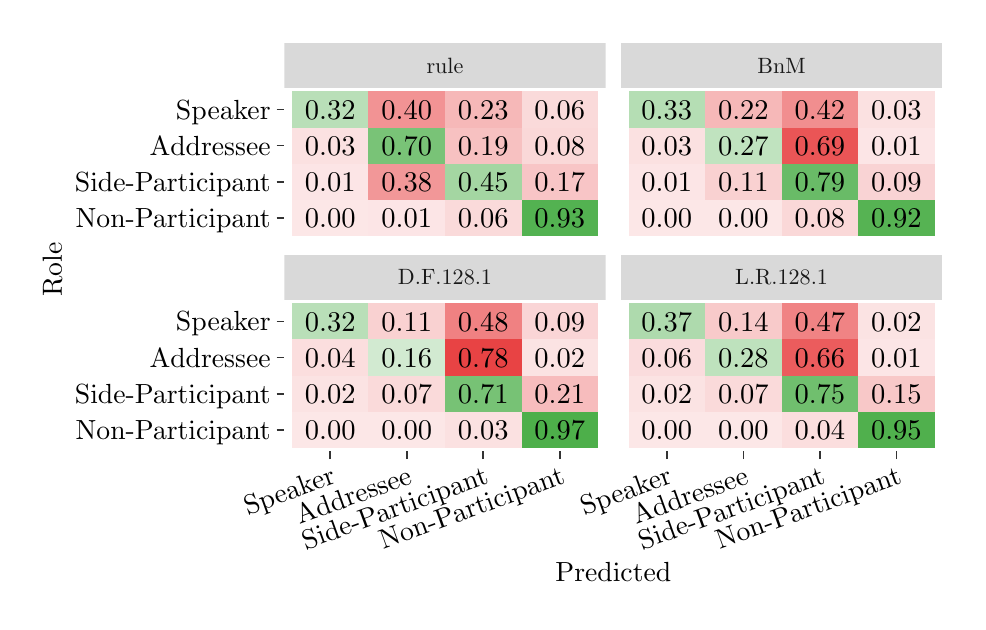
\begin{tikzpicture}[x=1pt,y=1pt]
\definecolor{fillColor}{RGB}{255,255,255}
\path[use as bounding box,fill=fillColor,fill opacity=0.00] (0,0) rectangle (336.00,207.65);
\begin{scope}
\path[clip] (  0.00,  0.00) rectangle (336.00,207.65);
\definecolor{drawColor}{RGB}{255,255,255}
\definecolor{fillColor}{RGB}{255,255,255}

\path[draw=drawColor,line width= 0.6pt,line join=round,line cap=round,fill=fillColor] (  0.00,  0.00) rectangle (336.00,207.65);
\end{scope}
\begin{scope}
\path[clip] ( 92.74,131.08) rectangle (208.87,185.89);
\definecolor{drawColor}{RGB}{255,255,255}

\path[draw=drawColor,line width= 0.6pt,line join=round] ( 92.74,138.91) --
	(208.87,138.91);

\path[draw=drawColor,line width= 0.6pt,line join=round] ( 92.74,151.96) --
	(208.87,151.96);

\path[draw=drawColor,line width= 0.6pt,line join=round] ( 92.74,165.01) --
	(208.87,165.01);

\path[draw=drawColor,line width= 0.6pt,line join=round] ( 92.74,178.06) --
	(208.87,178.06);

\path[draw=drawColor,line width= 0.6pt,line join=round] (109.33,131.08) --
	(109.33,185.89);

\path[draw=drawColor,line width= 0.6pt,line join=round] (136.98,131.08) --
	(136.98,185.89);

\path[draw=drawColor,line width= 0.6pt,line join=round] (164.63,131.08) --
	(164.63,185.89);

\path[draw=drawColor,line width= 0.6pt,line join=round] (192.28,131.08) --
	(192.28,185.89);
\definecolor{fillColor}{RGB}{77,175,74}

\path[fill=fillColor,fill opacity=0.39] ( 95.50,171.54) rectangle (123.15,184.59);
\definecolor{fillColor}{RGB}{228,26,28}

\path[fill=fillColor,fill opacity=0.47] (123.15,171.54) rectangle (150.80,184.59);
\definecolor{fillColor}{RGB}{228,26,28}

\path[fill=fillColor,fill opacity=0.31] (150.80,171.54) rectangle (178.45,184.59);
\definecolor{fillColor}{RGB}{228,26,28}

\path[fill=fillColor,fill opacity=0.16] (178.45,171.54) rectangle (206.10,184.59);
\definecolor{fillColor}{RGB}{228,26,28}

\path[fill=fillColor,fill opacity=0.13] ( 95.50,158.49) rectangle (123.15,171.54);
\definecolor{fillColor}{RGB}{77,175,74}

\path[fill=fillColor,fill opacity=0.75] (123.15,158.49) rectangle (150.80,171.54);
\definecolor{fillColor}{RGB}{228,26,28}

\path[fill=fillColor,fill opacity=0.27] (150.80,158.49) rectangle (178.45,171.54);
\definecolor{fillColor}{RGB}{228,26,28}

\path[fill=fillColor,fill opacity=0.17] (178.45,158.49) rectangle (206.10,171.54);
\definecolor{fillColor}{RGB}{228,26,28}

\path[fill=fillColor,fill opacity=0.11] ( 95.50,145.44) rectangle (123.15,158.49);
\definecolor{fillColor}{RGB}{228,26,28}

\path[fill=fillColor,fill opacity=0.45] (123.15,145.44) rectangle (150.80,158.49);
\definecolor{fillColor}{RGB}{77,175,74}

\path[fill=fillColor,fill opacity=0.51] (150.80,145.44) rectangle (178.45,158.49);
\definecolor{fillColor}{RGB}{228,26,28}

\path[fill=fillColor,fill opacity=0.25] (178.45,145.44) rectangle (206.10,158.49);
\definecolor{fillColor}{RGB}{228,26,28}

\path[fill=fillColor,fill opacity=0.10] ( 95.50,132.39) rectangle (123.15,145.44);
\definecolor{fillColor}{RGB}{228,26,28}

\path[fill=fillColor,fill opacity=0.11] (123.15,132.39) rectangle (150.80,145.44);
\definecolor{fillColor}{RGB}{228,26,28}

\path[fill=fillColor,fill opacity=0.16] (150.80,132.39) rectangle (178.45,145.44);
\definecolor{fillColor}{RGB}{77,175,74}

\path[fill=fillColor,fill opacity=0.96] (178.45,132.39) rectangle (206.10,145.44);
\definecolor{drawColor}{RGB}{0,0,0}

\node[text=drawColor,anchor=base,inner sep=0pt, outer sep=0pt, scale=  1.03] at (109.33,174.50) {0.32};

\node[text=drawColor,anchor=base,inner sep=0pt, outer sep=0pt, scale=  1.03] at (136.98,174.50) {0.40};

\node[text=drawColor,anchor=base,inner sep=0pt, outer sep=0pt, scale=  1.03] at (164.63,174.50) {0.23};

\node[text=drawColor,anchor=base,inner sep=0pt, outer sep=0pt, scale=  1.03] at (192.28,174.50) {0.06};

\node[text=drawColor,anchor=base,inner sep=0pt, outer sep=0pt, scale=  1.03] at (109.33,161.45) {0.03};

\node[text=drawColor,anchor=base,inner sep=0pt, outer sep=0pt, scale=  1.03] at (136.98,161.45) {0.70};

\node[text=drawColor,anchor=base,inner sep=0pt, outer sep=0pt, scale=  1.03] at (164.63,161.45) {0.19};

\node[text=drawColor,anchor=base,inner sep=0pt, outer sep=0pt, scale=  1.03] at (192.28,161.45) {0.08};

\node[text=drawColor,anchor=base,inner sep=0pt, outer sep=0pt, scale=  1.03] at (109.33,148.40) {0.01};

\node[text=drawColor,anchor=base,inner sep=0pt, outer sep=0pt, scale=  1.03] at (136.98,148.40) {0.38};

\node[text=drawColor,anchor=base,inner sep=0pt, outer sep=0pt, scale=  1.03] at (164.63,148.40) {0.45};

\node[text=drawColor,anchor=base,inner sep=0pt, outer sep=0pt, scale=  1.03] at (192.28,148.40) {0.17};

\node[text=drawColor,anchor=base,inner sep=0pt, outer sep=0pt, scale=  1.03] at (109.33,135.35) {0.00};

\node[text=drawColor,anchor=base,inner sep=0pt, outer sep=0pt, scale=  1.03] at (136.98,135.35) {0.01};

\node[text=drawColor,anchor=base,inner sep=0pt, outer sep=0pt, scale=  1.03] at (164.63,135.35) {0.06};

\node[text=drawColor,anchor=base,inner sep=0pt, outer sep=0pt, scale=  1.03] at (192.28,135.35) {0.93};
\end{scope}
\begin{scope}
\path[clip] ( 92.74, 54.51) rectangle (208.87,109.33);
\definecolor{drawColor}{RGB}{255,255,255}

\path[draw=drawColor,line width= 0.6pt,line join=round] ( 92.74, 62.34) --
	(208.87, 62.34);

\path[draw=drawColor,line width= 0.6pt,line join=round] ( 92.74, 75.39) --
	(208.87, 75.39);

\path[draw=drawColor,line width= 0.6pt,line join=round] ( 92.74, 88.44) --
	(208.87, 88.44);

\path[draw=drawColor,line width= 0.6pt,line join=round] ( 92.74,101.50) --
	(208.87,101.50);

\path[draw=drawColor,line width= 0.6pt,line join=round] (109.33, 54.51) --
	(109.33,109.33);

\path[draw=drawColor,line width= 0.6pt,line join=round] (136.98, 54.51) --
	(136.98,109.33);

\path[draw=drawColor,line width= 0.6pt,line join=round] (164.63, 54.51) --
	(164.63,109.33);

\path[draw=drawColor,line width= 0.6pt,line join=round] (192.28, 54.51) --
	(192.28,109.33);
\definecolor{fillColor}{RGB}{77,175,74}

\path[fill=fillColor,fill opacity=0.39] ( 95.50, 94.97) rectangle (123.15,108.02);
\definecolor{fillColor}{RGB}{228,26,28}

\path[fill=fillColor,fill opacity=0.20] (123.15, 94.97) rectangle (150.80,108.02);
\definecolor{fillColor}{RGB}{228,26,28}

\path[fill=fillColor,fill opacity=0.55] (150.80, 94.97) rectangle (178.45,108.02);
\definecolor{fillColor}{RGB}{228,26,28}

\path[fill=fillColor,fill opacity=0.18] (178.45, 94.97) rectangle (206.10,108.02);
\definecolor{fillColor}{RGB}{228,26,28}

\path[fill=fillColor,fill opacity=0.14] ( 95.50, 81.92) rectangle (123.15, 94.97);
\definecolor{fillColor}{RGB}{77,175,74}

\path[fill=fillColor,fill opacity=0.25] (123.15, 81.92) rectangle (150.80, 94.97);
\definecolor{fillColor}{RGB}{228,26,28}

\path[fill=fillColor,fill opacity=0.82] (150.80, 81.92) rectangle (178.45, 94.97);
\definecolor{fillColor}{RGB}{228,26,28}

\path[fill=fillColor,fill opacity=0.12] (178.45, 81.92) rectangle (206.10, 94.97);
\definecolor{fillColor}{RGB}{228,26,28}

\path[fill=fillColor,fill opacity=0.12] ( 95.50, 68.87) rectangle (123.15, 81.92);
\definecolor{fillColor}{RGB}{228,26,28}

\path[fill=fillColor,fill opacity=0.16] (123.15, 68.87) rectangle (150.80, 81.92);
\definecolor{fillColor}{RGB}{77,175,74}

\path[fill=fillColor,fill opacity=0.76] (150.80, 68.87) rectangle (178.45, 81.92);
\definecolor{fillColor}{RGB}{228,26,28}

\path[fill=fillColor,fill opacity=0.29] (178.45, 68.87) rectangle (206.10, 81.92);
\definecolor{fillColor}{RGB}{228,26,28}

\path[fill=fillColor,fill opacity=0.10] ( 95.50, 55.82) rectangle (123.15, 68.87);

\path[fill=fillColor,fill opacity=0.10] (123.15, 55.82) rectangle (150.80, 68.87);
\definecolor{fillColor}{RGB}{228,26,28}

\path[fill=fillColor,fill opacity=0.13] (150.80, 55.82) rectangle (178.45, 68.87);
\definecolor{fillColor}{RGB}{77,175,74}

\path[fill=fillColor] (178.45, 55.82) rectangle (206.10, 68.87);
\definecolor{drawColor}{RGB}{0,0,0}

\node[text=drawColor,anchor=base,inner sep=0pt, outer sep=0pt, scale=  1.03] at (109.33, 97.93) {0.32};

\node[text=drawColor,anchor=base,inner sep=0pt, outer sep=0pt, scale=  1.03] at (136.98, 97.93) {0.11};

\node[text=drawColor,anchor=base,inner sep=0pt, outer sep=0pt, scale=  1.03] at (164.63, 97.93) {0.48};

\node[text=drawColor,anchor=base,inner sep=0pt, outer sep=0pt, scale=  1.03] at (192.28, 97.93) {0.09};

\node[text=drawColor,anchor=base,inner sep=0pt, outer sep=0pt, scale=  1.03] at (109.33, 84.88) {0.04};

\node[text=drawColor,anchor=base,inner sep=0pt, outer sep=0pt, scale=  1.03] at (136.98, 84.88) {0.16};

\node[text=drawColor,anchor=base,inner sep=0pt, outer sep=0pt, scale=  1.03] at (164.63, 84.88) {0.78};

\node[text=drawColor,anchor=base,inner sep=0pt, outer sep=0pt, scale=  1.03] at (192.28, 84.88) {0.02};

\node[text=drawColor,anchor=base,inner sep=0pt, outer sep=0pt, scale=  1.03] at (109.33, 71.83) {0.02};

\node[text=drawColor,anchor=base,inner sep=0pt, outer sep=0pt, scale=  1.03] at (136.98, 71.83) {0.07};

\node[text=drawColor,anchor=base,inner sep=0pt, outer sep=0pt, scale=  1.03] at (164.63, 71.83) {0.71};

\node[text=drawColor,anchor=base,inner sep=0pt, outer sep=0pt, scale=  1.03] at (192.28, 71.83) {0.21};

\node[text=drawColor,anchor=base,inner sep=0pt, outer sep=0pt, scale=  1.03] at (109.33, 58.78) {0.00};

\node[text=drawColor,anchor=base,inner sep=0pt, outer sep=0pt, scale=  1.03] at (136.98, 58.78) {0.00};

\node[text=drawColor,anchor=base,inner sep=0pt, outer sep=0pt, scale=  1.03] at (164.63, 58.78) {0.03};

\node[text=drawColor,anchor=base,inner sep=0pt, outer sep=0pt, scale=  1.03] at (192.28, 58.78) {0.97};
\end{scope}
\begin{scope}
\path[clip] (214.37,131.08) rectangle (330.50,185.89);
\definecolor{drawColor}{RGB}{255,255,255}

\path[draw=drawColor,line width= 0.6pt,line join=round] (214.37,138.91) --
	(330.50,138.91);

\path[draw=drawColor,line width= 0.6pt,line join=round] (214.37,151.96) --
	(330.50,151.96);

\path[draw=drawColor,line width= 0.6pt,line join=round] (214.37,165.01) --
	(330.50,165.01);

\path[draw=drawColor,line width= 0.6pt,line join=round] (214.37,178.06) --
	(330.50,178.06);

\path[draw=drawColor,line width= 0.6pt,line join=round] (230.96,131.08) --
	(230.96,185.89);

\path[draw=drawColor,line width= 0.6pt,line join=round] (258.61,131.08) --
	(258.61,185.89);

\path[draw=drawColor,line width= 0.6pt,line join=round] (286.26,131.08) --
	(286.26,185.89);

\path[draw=drawColor,line width= 0.6pt,line join=round] (313.91,131.08) --
	(313.91,185.89);
\definecolor{fillColor}{RGB}{77,175,74}

\path[fill=fillColor,fill opacity=0.41] (217.13,171.54) rectangle (244.78,184.59);
\definecolor{fillColor}{RGB}{228,26,28}

\path[fill=fillColor,fill opacity=0.31] (244.78,171.54) rectangle (272.43,184.59);
\definecolor{fillColor}{RGB}{228,26,28}

\path[fill=fillColor,fill opacity=0.49] (272.43,171.54) rectangle (300.08,184.59);
\definecolor{fillColor}{RGB}{228,26,28}

\path[fill=fillColor,fill opacity=0.13] (300.08,171.54) rectangle (327.73,184.59);
\definecolor{fillColor}{RGB}{228,26,28}

\path[fill=fillColor,fill opacity=0.13] (217.13,158.49) rectangle (244.78,171.54);
\definecolor{fillColor}{RGB}{77,175,74}

\path[fill=fillColor,fill opacity=0.35] (244.78,158.49) rectangle (272.43,171.54);
\definecolor{fillColor}{RGB}{228,26,28}

\path[fill=fillColor,fill opacity=0.74] (272.43,158.49) rectangle (300.08,171.54);
\definecolor{fillColor}{RGB}{228,26,28}

\path[fill=fillColor,fill opacity=0.11] (300.08,158.49) rectangle (327.73,171.54);
\definecolor{fillColor}{RGB}{228,26,28}

\path[fill=fillColor,fill opacity=0.11] (217.13,145.44) rectangle (244.78,158.49);
\definecolor{fillColor}{RGB}{228,26,28}

\path[fill=fillColor,fill opacity=0.20] (244.78,145.44) rectangle (272.43,158.49);
\definecolor{fillColor}{RGB}{77,175,74}

\path[fill=fillColor,fill opacity=0.84] (272.43,145.44) rectangle (300.08,158.49);
\definecolor{fillColor}{RGB}{228,26,28}

\path[fill=fillColor,fill opacity=0.19] (300.08,145.44) rectangle (327.73,158.49);
\definecolor{fillColor}{RGB}{228,26,28}

\path[fill=fillColor,fill opacity=0.10] (217.13,132.39) rectangle (244.78,145.44);

\path[fill=fillColor,fill opacity=0.10] (244.78,132.39) rectangle (272.43,145.44);
\definecolor{fillColor}{RGB}{228,26,28}

\path[fill=fillColor,fill opacity=0.17] (272.43,132.39) rectangle (300.08,145.44);
\definecolor{fillColor}{RGB}{77,175,74}

\path[fill=fillColor,fill opacity=0.95] (300.08,132.39) rectangle (327.73,145.44);
\definecolor{drawColor}{RGB}{0,0,0}

\node[text=drawColor,anchor=base,inner sep=0pt, outer sep=0pt, scale=  1.03] at (230.96,174.50) {0.33};

\node[text=drawColor,anchor=base,inner sep=0pt, outer sep=0pt, scale=  1.03] at (258.61,174.50) {0.22};

\node[text=drawColor,anchor=base,inner sep=0pt, outer sep=0pt, scale=  1.03] at (286.26,174.50) {0.42};

\node[text=drawColor,anchor=base,inner sep=0pt, outer sep=0pt, scale=  1.03] at (313.91,174.50) {0.03};

\node[text=drawColor,anchor=base,inner sep=0pt, outer sep=0pt, scale=  1.03] at (230.96,161.45) {0.03};

\node[text=drawColor,anchor=base,inner sep=0pt, outer sep=0pt, scale=  1.03] at (258.61,161.45) {0.27};

\node[text=drawColor,anchor=base,inner sep=0pt, outer sep=0pt, scale=  1.03] at (286.26,161.45) {0.69};

\node[text=drawColor,anchor=base,inner sep=0pt, outer sep=0pt, scale=  1.03] at (313.91,161.45) {0.01};

\node[text=drawColor,anchor=base,inner sep=0pt, outer sep=0pt, scale=  1.03] at (230.96,148.40) {0.01};

\node[text=drawColor,anchor=base,inner sep=0pt, outer sep=0pt, scale=  1.03] at (258.61,148.40) {0.11};

\node[text=drawColor,anchor=base,inner sep=0pt, outer sep=0pt, scale=  1.03] at (286.26,148.40) {0.79};

\node[text=drawColor,anchor=base,inner sep=0pt, outer sep=0pt, scale=  1.03] at (313.91,148.40) {0.09};

\node[text=drawColor,anchor=base,inner sep=0pt, outer sep=0pt, scale=  1.03] at (230.96,135.35) {0.00};

\node[text=drawColor,anchor=base,inner sep=0pt, outer sep=0pt, scale=  1.03] at (258.61,135.35) {0.00};

\node[text=drawColor,anchor=base,inner sep=0pt, outer sep=0pt, scale=  1.03] at (286.26,135.35) {0.08};

\node[text=drawColor,anchor=base,inner sep=0pt, outer sep=0pt, scale=  1.03] at (313.91,135.35) {0.92};
\end{scope}
\begin{scope}
\path[clip] (214.37, 54.51) rectangle (330.50,109.33);
\definecolor{drawColor}{RGB}{255,255,255}

\path[draw=drawColor,line width= 0.6pt,line join=round] (214.37, 62.34) --
	(330.50, 62.34);

\path[draw=drawColor,line width= 0.6pt,line join=round] (214.37, 75.39) --
	(330.50, 75.39);

\path[draw=drawColor,line width= 0.6pt,line join=round] (214.37, 88.44) --
	(330.50, 88.44);

\path[draw=drawColor,line width= 0.6pt,line join=round] (214.37,101.50) --
	(330.50,101.50);

\path[draw=drawColor,line width= 0.6pt,line join=round] (230.96, 54.51) --
	(230.96,109.33);

\path[draw=drawColor,line width= 0.6pt,line join=round] (258.61, 54.51) --
	(258.61,109.33);

\path[draw=drawColor,line width= 0.6pt,line join=round] (286.26, 54.51) --
	(286.26,109.33);

\path[draw=drawColor,line width= 0.6pt,line join=round] (313.91, 54.51) --
	(313.91,109.33);
\definecolor{fillColor}{RGB}{77,175,74}

\path[fill=fillColor,fill opacity=0.45] (217.13, 94.97) rectangle (244.78,108.02);
\definecolor{fillColor}{RGB}{228,26,28}

\path[fill=fillColor,fill opacity=0.23] (244.78, 94.97) rectangle (272.43,108.02);
\definecolor{fillColor}{RGB}{228,26,28}

\path[fill=fillColor,fill opacity=0.54] (272.43, 94.97) rectangle (300.08,108.02);
\definecolor{fillColor}{RGB}{228,26,28}

\path[fill=fillColor,fill opacity=0.12] (300.08, 94.97) rectangle (327.73,108.02);
\definecolor{fillColor}{RGB}{228,26,28}

\path[fill=fillColor,fill opacity=0.15] (217.13, 81.92) rectangle (244.78, 94.97);
\definecolor{fillColor}{RGB}{77,175,74}

\path[fill=fillColor,fill opacity=0.36] (244.78, 81.92) rectangle (272.43, 94.97);
\definecolor{fillColor}{RGB}{228,26,28}

\path[fill=fillColor,fill opacity=0.71] (272.43, 81.92) rectangle (300.08, 94.97);
\definecolor{fillColor}{RGB}{228,26,28}

\path[fill=fillColor,fill opacity=0.11] (300.08, 81.92) rectangle (327.73, 94.97);
\definecolor{fillColor}{RGB}{228,26,28}

\path[fill=fillColor,fill opacity=0.12] (217.13, 68.87) rectangle (244.78, 81.92);
\definecolor{fillColor}{RGB}{228,26,28}

\path[fill=fillColor,fill opacity=0.16] (244.78, 68.87) rectangle (272.43, 81.92);
\definecolor{fillColor}{RGB}{77,175,74}

\path[fill=fillColor,fill opacity=0.80] (272.43, 68.87) rectangle (300.08, 81.92);
\definecolor{fillColor}{RGB}{228,26,28}

\path[fill=fillColor,fill opacity=0.24] (300.08, 68.87) rectangle (327.73, 81.92);
\definecolor{fillColor}{RGB}{228,26,28}

\path[fill=fillColor,fill opacity=0.10] (217.13, 55.82) rectangle (244.78, 68.87);

\path[fill=fillColor,fill opacity=0.10] (244.78, 55.82) rectangle (272.43, 68.87);
\definecolor{fillColor}{RGB}{228,26,28}

\path[fill=fillColor,fill opacity=0.14] (272.43, 55.82) rectangle (300.08, 68.87);
\definecolor{fillColor}{RGB}{77,175,74}

\path[fill=fillColor,fill opacity=0.98] (300.08, 55.82) rectangle (327.73, 68.87);
\definecolor{drawColor}{RGB}{0,0,0}

\node[text=drawColor,anchor=base,inner sep=0pt, outer sep=0pt, scale=  1.03] at (230.96, 97.93) {0.37};

\node[text=drawColor,anchor=base,inner sep=0pt, outer sep=0pt, scale=  1.03] at (258.61, 97.93) {0.14};

\node[text=drawColor,anchor=base,inner sep=0pt, outer sep=0pt, scale=  1.03] at (286.26, 97.93) {0.47};

\node[text=drawColor,anchor=base,inner sep=0pt, outer sep=0pt, scale=  1.03] at (313.91, 97.93) {0.02};

\node[text=drawColor,anchor=base,inner sep=0pt, outer sep=0pt, scale=  1.03] at (230.96, 84.88) {0.06};

\node[text=drawColor,anchor=base,inner sep=0pt, outer sep=0pt, scale=  1.03] at (258.61, 84.88) {0.28};

\node[text=drawColor,anchor=base,inner sep=0pt, outer sep=0pt, scale=  1.03] at (286.26, 84.88) {0.66};

\node[text=drawColor,anchor=base,inner sep=0pt, outer sep=0pt, scale=  1.03] at (313.91, 84.88) {0.01};

\node[text=drawColor,anchor=base,inner sep=0pt, outer sep=0pt, scale=  1.03] at (230.96, 71.83) {0.02};

\node[text=drawColor,anchor=base,inner sep=0pt, outer sep=0pt, scale=  1.03] at (258.61, 71.83) {0.07};

\node[text=drawColor,anchor=base,inner sep=0pt, outer sep=0pt, scale=  1.03] at (286.26, 71.83) {0.75};

\node[text=drawColor,anchor=base,inner sep=0pt, outer sep=0pt, scale=  1.03] at (313.91, 71.83) {0.15};

\node[text=drawColor,anchor=base,inner sep=0pt, outer sep=0pt, scale=  1.03] at (230.96, 58.78) {0.00};

\node[text=drawColor,anchor=base,inner sep=0pt, outer sep=0pt, scale=  1.03] at (258.61, 58.78) {0.00};

\node[text=drawColor,anchor=base,inner sep=0pt, outer sep=0pt, scale=  1.03] at (286.26, 58.78) {0.04};

\node[text=drawColor,anchor=base,inner sep=0pt, outer sep=0pt, scale=  1.03] at (313.91, 58.78) {0.95};
\end{scope}
\begin{scope}
\path[clip] ( 92.74,109.33) rectangle (208.87,125.58);
\definecolor{fillColor}{gray}{0.85}

\path[fill=fillColor] ( 92.74,109.33) rectangle (208.87,125.58);
\definecolor{drawColor}{gray}{0.10}

\node[text=drawColor,anchor=base,inner sep=0pt, outer sep=0pt, scale=  0.80] at (150.80,114.70) {D.F.128.1};
\end{scope}
\begin{scope}
\path[clip] (214.37,109.33) rectangle (330.50,125.58);
\definecolor{fillColor}{gray}{0.85}

\path[fill=fillColor] (214.37,109.33) rectangle (330.50,125.58);
\definecolor{drawColor}{gray}{0.10}

\node[text=drawColor,anchor=base,inner sep=0pt, outer sep=0pt, scale=  0.80] at (272.43,114.70) {L.R.128.1};
\end{scope}
\begin{scope}
\path[clip] ( 92.74,185.89) rectangle (208.87,202.15);
\definecolor{fillColor}{gray}{0.85}

\path[fill=fillColor] ( 92.74,185.89) rectangle (208.87,202.15);
\definecolor{drawColor}{gray}{0.10}

\node[text=drawColor,anchor=base,inner sep=0pt, outer sep=0pt, scale=  0.80] at (150.80,191.27) {rule};
\end{scope}
\begin{scope}
\path[clip] (214.37,185.89) rectangle (330.50,202.15);
\definecolor{fillColor}{gray}{0.85}

\path[fill=fillColor] (214.37,185.89) rectangle (330.50,202.15);
\definecolor{drawColor}{gray}{0.10}

\node[text=drawColor,anchor=base,inner sep=0pt, outer sep=0pt, scale=  0.80] at (272.43,191.27) {BnM};
\end{scope}
\begin{scope}
\path[clip] (  0.00,  0.00) rectangle (336.00,207.65);
\definecolor{drawColor}{gray}{0.20}

\path[draw=drawColor,line width= 0.6pt,line join=round] (109.33, 51.76) --
	(109.33, 54.51);

\path[draw=drawColor,line width= 0.6pt,line join=round] (136.98, 51.76) --
	(136.98, 54.51);

\path[draw=drawColor,line width= 0.6pt,line join=round] (164.63, 51.76) --
	(164.63, 54.51);

\path[draw=drawColor,line width= 0.6pt,line join=round] (192.28, 51.76) --
	(192.28, 54.51);
\end{scope}
\begin{scope}
\path[clip] (  0.00,  0.00) rectangle (336.00,207.65);
\definecolor{drawColor}{RGB}{0,0,0}

\node[text=drawColor,rotate= 20.00,anchor=base east,inner sep=0pt, outer sep=0pt, scale=  1.00] at (111.68, 43.09) {Speaker};

\node[text=drawColor,rotate= 20.00,anchor=base east,inner sep=0pt, outer sep=0pt, scale=  1.00] at (139.33, 43.09) {Addressee};

\node[text=drawColor,rotate= 20.00,anchor=base east,inner sep=0pt, outer sep=0pt, scale=  1.00] at (166.98, 43.09) {Side-Participant};

\node[text=drawColor,rotate= 20.00,anchor=base east,inner sep=0pt, outer sep=0pt, scale=  1.00] at (194.63, 43.09) {Non-Participant};
\end{scope}
\begin{scope}
\path[clip] (  0.00,  0.00) rectangle (336.00,207.65);
\definecolor{drawColor}{gray}{0.20}

\path[draw=drawColor,line width= 0.6pt,line join=round] (230.96, 51.76) --
	(230.96, 54.51);

\path[draw=drawColor,line width= 0.6pt,line join=round] (258.61, 51.76) --
	(258.61, 54.51);

\path[draw=drawColor,line width= 0.6pt,line join=round] (286.26, 51.76) --
	(286.26, 54.51);

\path[draw=drawColor,line width= 0.6pt,line join=round] (313.91, 51.76) --
	(313.91, 54.51);
\end{scope}
\begin{scope}
\path[clip] (  0.00,  0.00) rectangle (336.00,207.65);
\definecolor{drawColor}{RGB}{0,0,0}

\node[text=drawColor,rotate= 20.00,anchor=base east,inner sep=0pt, outer sep=0pt, scale=  1.00] at (233.31, 43.09) {Speaker};

\node[text=drawColor,rotate= 20.00,anchor=base east,inner sep=0pt, outer sep=0pt, scale=  1.00] at (260.96, 43.09) {Addressee};

\node[text=drawColor,rotate= 20.00,anchor=base east,inner sep=0pt, outer sep=0pt, scale=  1.00] at (288.61, 43.09) {Side-Participant};

\node[text=drawColor,rotate= 20.00,anchor=base east,inner sep=0pt, outer sep=0pt, scale=  1.00] at (316.27, 43.09) {Non-Participant};
\end{scope}
\begin{scope}
\path[clip] (  0.00,  0.00) rectangle (336.00,207.65);
\definecolor{drawColor}{RGB}{0,0,0}

\node[text=drawColor,anchor=base east,inner sep=0pt, outer sep=0pt, scale=  1.00] at ( 87.79,135.47) {Non-Participant};

\node[text=drawColor,anchor=base east,inner sep=0pt, outer sep=0pt, scale=  1.00] at ( 87.79,148.52) {Side-Participant};

\node[text=drawColor,anchor=base east,inner sep=0pt, outer sep=0pt, scale=  1.00] at ( 87.79,161.57) {Addressee};

\node[text=drawColor,anchor=base east,inner sep=0pt, outer sep=0pt, scale=  1.00] at ( 87.79,174.62) {Speaker};
\end{scope}
\begin{scope}
\path[clip] (  0.00,  0.00) rectangle (336.00,207.65);
\definecolor{drawColor}{gray}{0.20}

\path[draw=drawColor,line width= 0.6pt,line join=round] ( 89.99,138.91) --
	( 92.74,138.91);

\path[draw=drawColor,line width= 0.6pt,line join=round] ( 89.99,151.96) --
	( 92.74,151.96);

\path[draw=drawColor,line width= 0.6pt,line join=round] ( 89.99,165.01) --
	( 92.74,165.01);

\path[draw=drawColor,line width= 0.6pt,line join=round] ( 89.99,178.06) --
	( 92.74,178.06);
\end{scope}
\begin{scope}
\path[clip] (  0.00,  0.00) rectangle (336.00,207.65);
\definecolor{drawColor}{RGB}{0,0,0}

\node[text=drawColor,anchor=base east,inner sep=0pt, outer sep=0pt, scale=  1.00] at ( 87.79, 58.90) {Non-Participant};

\node[text=drawColor,anchor=base east,inner sep=0pt, outer sep=0pt, scale=  1.00] at ( 87.79, 71.95) {Side-Participant};

\node[text=drawColor,anchor=base east,inner sep=0pt, outer sep=0pt, scale=  1.00] at ( 87.79, 85.00) {Addressee};

\node[text=drawColor,anchor=base east,inner sep=0pt, outer sep=0pt, scale=  1.00] at ( 87.79, 98.05) {Speaker};
\end{scope}
\begin{scope}
\path[clip] (  0.00,  0.00) rectangle (336.00,207.65);
\definecolor{drawColor}{gray}{0.20}

\path[draw=drawColor,line width= 0.6pt,line join=round] ( 89.99, 62.34) --
	( 92.74, 62.34);

\path[draw=drawColor,line width= 0.6pt,line join=round] ( 89.99, 75.39) --
	( 92.74, 75.39);

\path[draw=drawColor,line width= 0.6pt,line join=round] ( 89.99, 88.44) --
	( 92.74, 88.44);

\path[draw=drawColor,line width= 0.6pt,line join=round] ( 89.99,101.50) --
	( 92.74,101.50);
\end{scope}
\begin{scope}
\path[clip] (  0.00,  0.00) rectangle (336.00,207.65);
\definecolor{drawColor}{RGB}{0,0,0}

\node[text=drawColor,anchor=base,inner sep=0pt, outer sep=0pt, scale=  1.00] at (211.62,  7.44) {Predicted};
\end{scope}
\begin{scope}
\path[clip] (  0.00,  0.00) rectangle (336.00,207.65);
\definecolor{drawColor}{RGB}{0,0,0}

\node[text=drawColor,rotate= 90.00,anchor=base,inner sep=0pt, outer sep=0pt, scale=  1.00] at ( 12.39,120.20) {Role};
\end{scope}
\end{tikzpicture}
